%!TEX root = ../../../exa-ma-d7.1.tex
\section{Software: \texorpdfstring{\Feelpp}{Feel++}}
\label{sec:WP1:Feelpp:software}

\begin{table}[!ht]
    \centering
    { \setlength{\parindent}{0pt}
    \def\arraystretch{1.25}
    \arrayrulecolor{numpexgray}
    {\fontsize{9}{11}\selectfont
    \begin{tabular}{!{\color{numpexgray}\vrule}p{.4\textwidth}!{\color{numpexgray}\vrule}p{.6\textwidth}!{\color{numpexgray}\vrule}}
        \rowcolor{numpexgray}{\rule{0pt}{2.5ex}\color{white}\bf Field} & {\rule{0pt}{2.5ex}\color{white}\bf Details} \\
        \rowcolor{white}\textbf{Consortium} & \begin{tabular}{l}
\Feelpp{} Consortium\\
\end{tabular} \\
        \rowcolor{numpexlightergray}\textbf{Exa-MA Partners} & \begin{tabular}{l}
CNRS\\
Inria Grenoble\\
Unistra\\
\end{tabular} \\
        \rowcolor{white}\textbf{Contact Emails} & \begin{tabular}{l}
christophe.prudhomme@cemosis.fr\\
vincent.chabannes@cemosis.fr\\
\end{tabular} \\
        \rowcolor{numpexlightergray}\textbf{Supported Architectures} & \begin{tabular}{l}
CPU Only\\
\end{tabular} \\
        \rowcolor{white}\textbf{Repository} & \href{https://github.com/feelpp/feelpp}{https://github.com/feelpp/feelpp} \\
        \rowcolor{numpexlightergray}\textbf{License} & \begin{tabular}{l}
OSS:: GPL v*\\
OSS:: LGPL v*\\
\end{tabular} \\
        \rowcolor{white}\textbf{Bottlenecks roadmap} & \begin{tabular}{l}
B10 - Scientific Productivity\\
B11 - Reproducibility and Replicability of Computation\\
B12 - Pre/Post Processing and In-Situ Processing\\
B2 - Interconnect Technology\\
B6 - Data Management\\
B7 - Exascale Algorithms\\
\end{tabular} \\
\rowcolor{numpexlightergray}\textbf{Contributors} & \begin{tabular}{l}
    Christophe Prud'homme (UNISTRA)\\
    Vincent Chabannes (UNISTRA)\\
    Thomas Saigre (UNISTRA)\\
    Céline Van Landeghem (UNISTRA)\\
    Christophe Trophime (CNRS)\\
\end{tabular}\\
        \hline
    \end{tabular}
    }}
    \caption{WP1: \Feelpp{} Information}
\end{table}

\subsection{Software Overview}
\label{sec:WP1:Feelpp:summary}

\Feelpp is an open-source \Cpp{} library designed for solving partial differential equations (PDEs), it supports seamless parallel computing based on MPI, and it is designed to be highly modular and extensible.
It implements a \ac{DSEL} for variational formulations, which allows users to define complex PDEs in a concise and readable manner directly in \Cpp{} leveraging the power of modern \Cpp{} features.

In~\Cref{tab:WP1:Feelpp:features} we provide a summary of the software features relevant to the work package which are briefly discussed.

\begin{table}[!ht]
    \centering
    {
        \setlength{\parindent}{0pt}
        \def\arraystretch{1.25}
        \arrayrulecolor{numpexgray}
        {
            \fontsize{9}{11}\selectfont
            \begin{tabular}{!{\color{numpexgray}\vrule}p{.25\linewidth}!{\color{numpexgray}\vrule}p{.6885\linewidth}!{\color{numpexgray}\vrule}}

    \rowcolor{numpexgray}{\rule{0pt}{2.5ex}\color{white}\bf Features} &  {\rule{0pt}{2.5ex}\color{white}\bf Short Description }\\

\rowcolor{white}    cG&  continuous Galerkin of arbitrary order; conforming and non conforming interpolation operator;  \ac{DSEL} for cG methods and variational formulations \\
\rowcolor{numpexlightergray}    dG/hdG & support dG and HdG methods in 1D, 2D and 3D of arbitrary order; support postprocessing for increased accuracy for HdG; Static condensation multithreaded; \ac{DSEL} for dG/HdG methods and variational formulations\\
\rowcolor{white}    finite element & $H^1$, $L^2$, $H^\mathrm{div}$ and $H^\mathrm{curl}$ finite elements of arbitrary order in 1D, 2D, 3D; \\
\rowcolor{numpexlightergray}    inhouse & efficient data structures for localisation: BVH and KD-trees \\
\rowcolor{white}    interface & interfaces with MMG/ParMMG; Gmsh; Eigen3 \\
\rowcolor{numpexlightergray}    mesh adaptation & use MMG and ParMMG for mesh adaptation; mesh quality indicators to trigger adaptation\\
\rowcolor{white}    multiphysics coupling & Support for function space cartesian products; \ac{DSEL} for variational formulations  \\
\rowcolor{numpexlightergray}    multiscale coupling & multi-dimension coupling, \textit{e.g.} 0D-3D, 1D-3D or 2D-3D; support for solving coupled systems of PDEs and ODEs\\
\rowcolor{white}    parallel in time & space-time parallel implementation of original parareal algorithm \\
\rowcolor{numpexlightergray}    spectral element & high order methods on simplices and hypercubes; Gauss-Legendre, Gauss-Lobatto, Gauss-Radau, electrostatic and Fekete points;  high order geometric transformation (up to order 4 using Gmsh); construction of $P_N \mathrm{iso} P_1$; $L^2$ orthonormal basis functions used as primal basis functions on hypercubes (Gauss-Legendre) and simplices (Dubiner) \\
\rowcolor{white}    unstructured mesh & Hypercubes and Simplices meshes in 1D, 2D and 3D as well as 1D meshes in 2D and 3D and 2D meshes in 3D; efficient localisation using kd-tree; \ac{DSEL} to manipulate geometric entity collections (points,edges,faces, facets and volumes)\\
\hline
\end{tabular}
        }
    }
    \caption{WP1: \Feelpp Features}
    \label{tab:WP1:Feelpp:features}
\end{table}


\subsection{Parallel Capabilities}
\label{sec:WP1:Feelpp:performances}


\begin{itemize}
    \item describe the parallel programming  environment : MPI, OpenMP, CUDA, OpenACC, etc.
    \item describe the parallel computation environment: type of architecture and super computer used.
    \item describe the parallel capabilities of the software
    \item \textbf{Scalability:} Describe the general scalability properties of the software
    \item \textbf{Integration with Other Systems:} Describe how the software integrates with other numerical libraries in the Exa-MA framework.
\end{itemize}


\subsection{Initial Performance Metrics}
\label{sec:WP1:Feelpp:metrics}

This section provides a summary of initial performance benchmarks performed in the context of WP1. It ensures reproducibility by detailing input/output datasets, benchmarking tools, and the results. All data should be publicly available, ideally with a DOI for future reference.

\begin{itemize}
    \item \textbf{Overall Performance:} Summarize the software's computational performance, energy efficiency, and scalability results across different architectures (e.g., CPU, GPU, hybrid systems).
    \item \textbf{Input/Output Dataset:} Provide a detailed description of the dataset used for the benchmark, including:
        \begin{itemize}
            \item Input dataset size, structure, and format (e.g., CSV, HDF5, NetCDF).
            \item Output dataset format and key results.
            \item Location of the dataset (e.g., GitHub repository, institutional repository, or open access platform).
            \item DOI or permanent link for accessing the dataset.
        \end{itemize}
    \item \textbf{open-data Access:} Indicate whether the datasets used for the benchmark are open access, and provide a DOI or a direct link for download. Where applicable, highlight any licensing constraints.
    \item \textbf{Challenges:} Identify any significant bottlenecks or challenges observed during the benchmarking process, including data handling and computational performance.
    \item \textbf{Future Improvements:} Outline areas for optimization, including dataset handling, memory usage, or algorithmic efficiency, to address identified challenges.
\end{itemize}

\subsubsection{Benchmark \#1: Compute Distance Function}

\paragraph{Description}
This benchmark evaluates two methods for computing the distance function inside a three-dimensional box:
\begin{enumerate}
    \item The \textbf{Level Set} method using the \textbf{Fast Marching Algorithm (FMA)}.
    \item The \textbf{Ray Tracing} method.
\end{enumerate}
The objective is to compute the distance function at all vertices of a discretized box using both methods and verify whether they produce the same results.
The problem is discretized using an unstructured grid, and performance is assessed on a multi-core CPU architecture.

The benchmark aims to compare the efficiency, accuracy, and computational cost of both approaches in terms of distance calculation within the 3D domain.

\paragraph{Benchmarking Tools Used}
The following tools were used for performance profiling and analysis:
\begin{itemize}
\item \textbf{\Feelpp}: the performance tools integrated into the \Feelpp framework were used to measure the execution time.
\end{itemize}

The key metrics measured include execution time, accuracy, memory usage, and floating-point operations (FLOPS) for both methods.

\subsection{Input/Output Dataset Description}
\begin{itemize}
    \item \textbf{Input Data:} The input consists of a 3D uniform grid representing the box geometry, with approximately 1 million vertices. The level set function and ray tracing boundaries are initialized for the distance computation. The input data is stored in JSON format, and it can be accessed via DOI: \texttt{[Insert DOI]}.

    \item \textbf{Output Data:} The output includes the computed distance function values at all vertices for both methods, stored in CSV format. Additionally, runtime performance logs and accuracy comparisons between the methods are included.

    \item \textbf{Data Repository:} Input and output datasets, along with performance logs, are stored in a Zenodo repository and can be accessed via DOI: \texttt{[Insert DOI]}.
\end{itemize}

\paragraph{Results Summary}
The performance comparison between the two methods is summarized as follows:

RESULTS here.

\paragraph{Challenges Identified}
The following challenges were encountered during the benchmarking process:
\begin{itemize}
    \item \textbf{Ray Tracing Bottlenecks:}
    \item \textbf{Parallelization Issues:}
    \item \textbf{Memory Usage:}
\end{itemize}

Final analysis and persectives here.

\begin{itemize}
    \item \textbf{Description:} Briefly describe the benchmark case, including the problem size, target architecture (e.g., CPU, GPU), and the input data. Mention the specific goals of the benchmark (e.g., testing scalability, energy efficiency).
    \item \textbf{Benchmarking Tools Used:} List the tools used for performance analysis, such as Extrae, Score-P, TAU, Vampir, or Nsight, and specify what metrics were measured (e.g., execution time, FLOPS, energy consumption).
    \item \textbf{Input/Output Dataset Description:}
        \begin{itemize}
            \item \textbf{Input Data:} Describe the input dataset (size, format, data type) and provide a DOI or link to access it.
            \item \textbf{Output Data:} Specify the structure of the results (e.g., memory usage, runtime logs) and how they can be accessed or replicated.
            \item \textbf{Data Repository:} Indicate where the data is stored (e.g., Zenodo, institutional repository) and provide a DOI or URL for accessing the data.
        \end{itemize}
    \item \textbf{Results Summary:} Include a summary of key metrics (execution time, memory usage, FLOPS) and their comparison across architectures (e.g., CPU, GPU).
    \item \textbf{Challenges Identified:} Describe any bottlenecks encountered (e.g., memory usage, parallelization inefficiencies) and how they impacted the benchmark.
\end{itemize}

\subsubsection{Benchmark \#2: Elliptic linear PDE : Thermal bridges}
\label{sec:WP1:Feelpp:benchmark:thermal_bridges}
\paragraph{Description:} %Briefly describe the benchmark case, including the problem size, target architecture (e.g., CPU, GPU), and the input data. Mention the specific goals of the benchmark (e.g., testing scalability, energy efficiency).

The benchmark known as "thermal bridges" is an example of an application that
enables us to validate numerical simulation tools using \Feelpp. We have
developed tests based on the ISO 10211:2017 standard
\fullcite{noauthor_iso_2017}, which provides methodologies for evaluating
thermal bridges in building construction.

Thermal bridges are areas within a building envelope where heat
flow is different compared to adjacent areas, often resulting in increased heat
loss or unwanted condensation.
The standard is intended to ensure that thermal
bridges simulation are accurately computed. It provides reference values (and tolerance) on heat
temperature and heat flux at several location of the geometry.

At the mathematical level, this application requires finding the numerical
solution of an elliptic linear PDE (i.e. the heat equation). We employ a
finite element method based on continuous Lagrange Finite Element of order 1,2
and 3 (denoted by $P_1$,$P_2$,$P_3$). And we analyzed the execution time of the
main components of the simulation.

The \Cref{fig:wp1:feelpp:thermal_bridges:visualization} illustrate the geometry
used, the 3D temperature field solution, and an example of mesh partitioning.


\begin{figure}[h]
  \centering
  \begin{subfigure}[c]{0.49\textwidth}
    \centering
    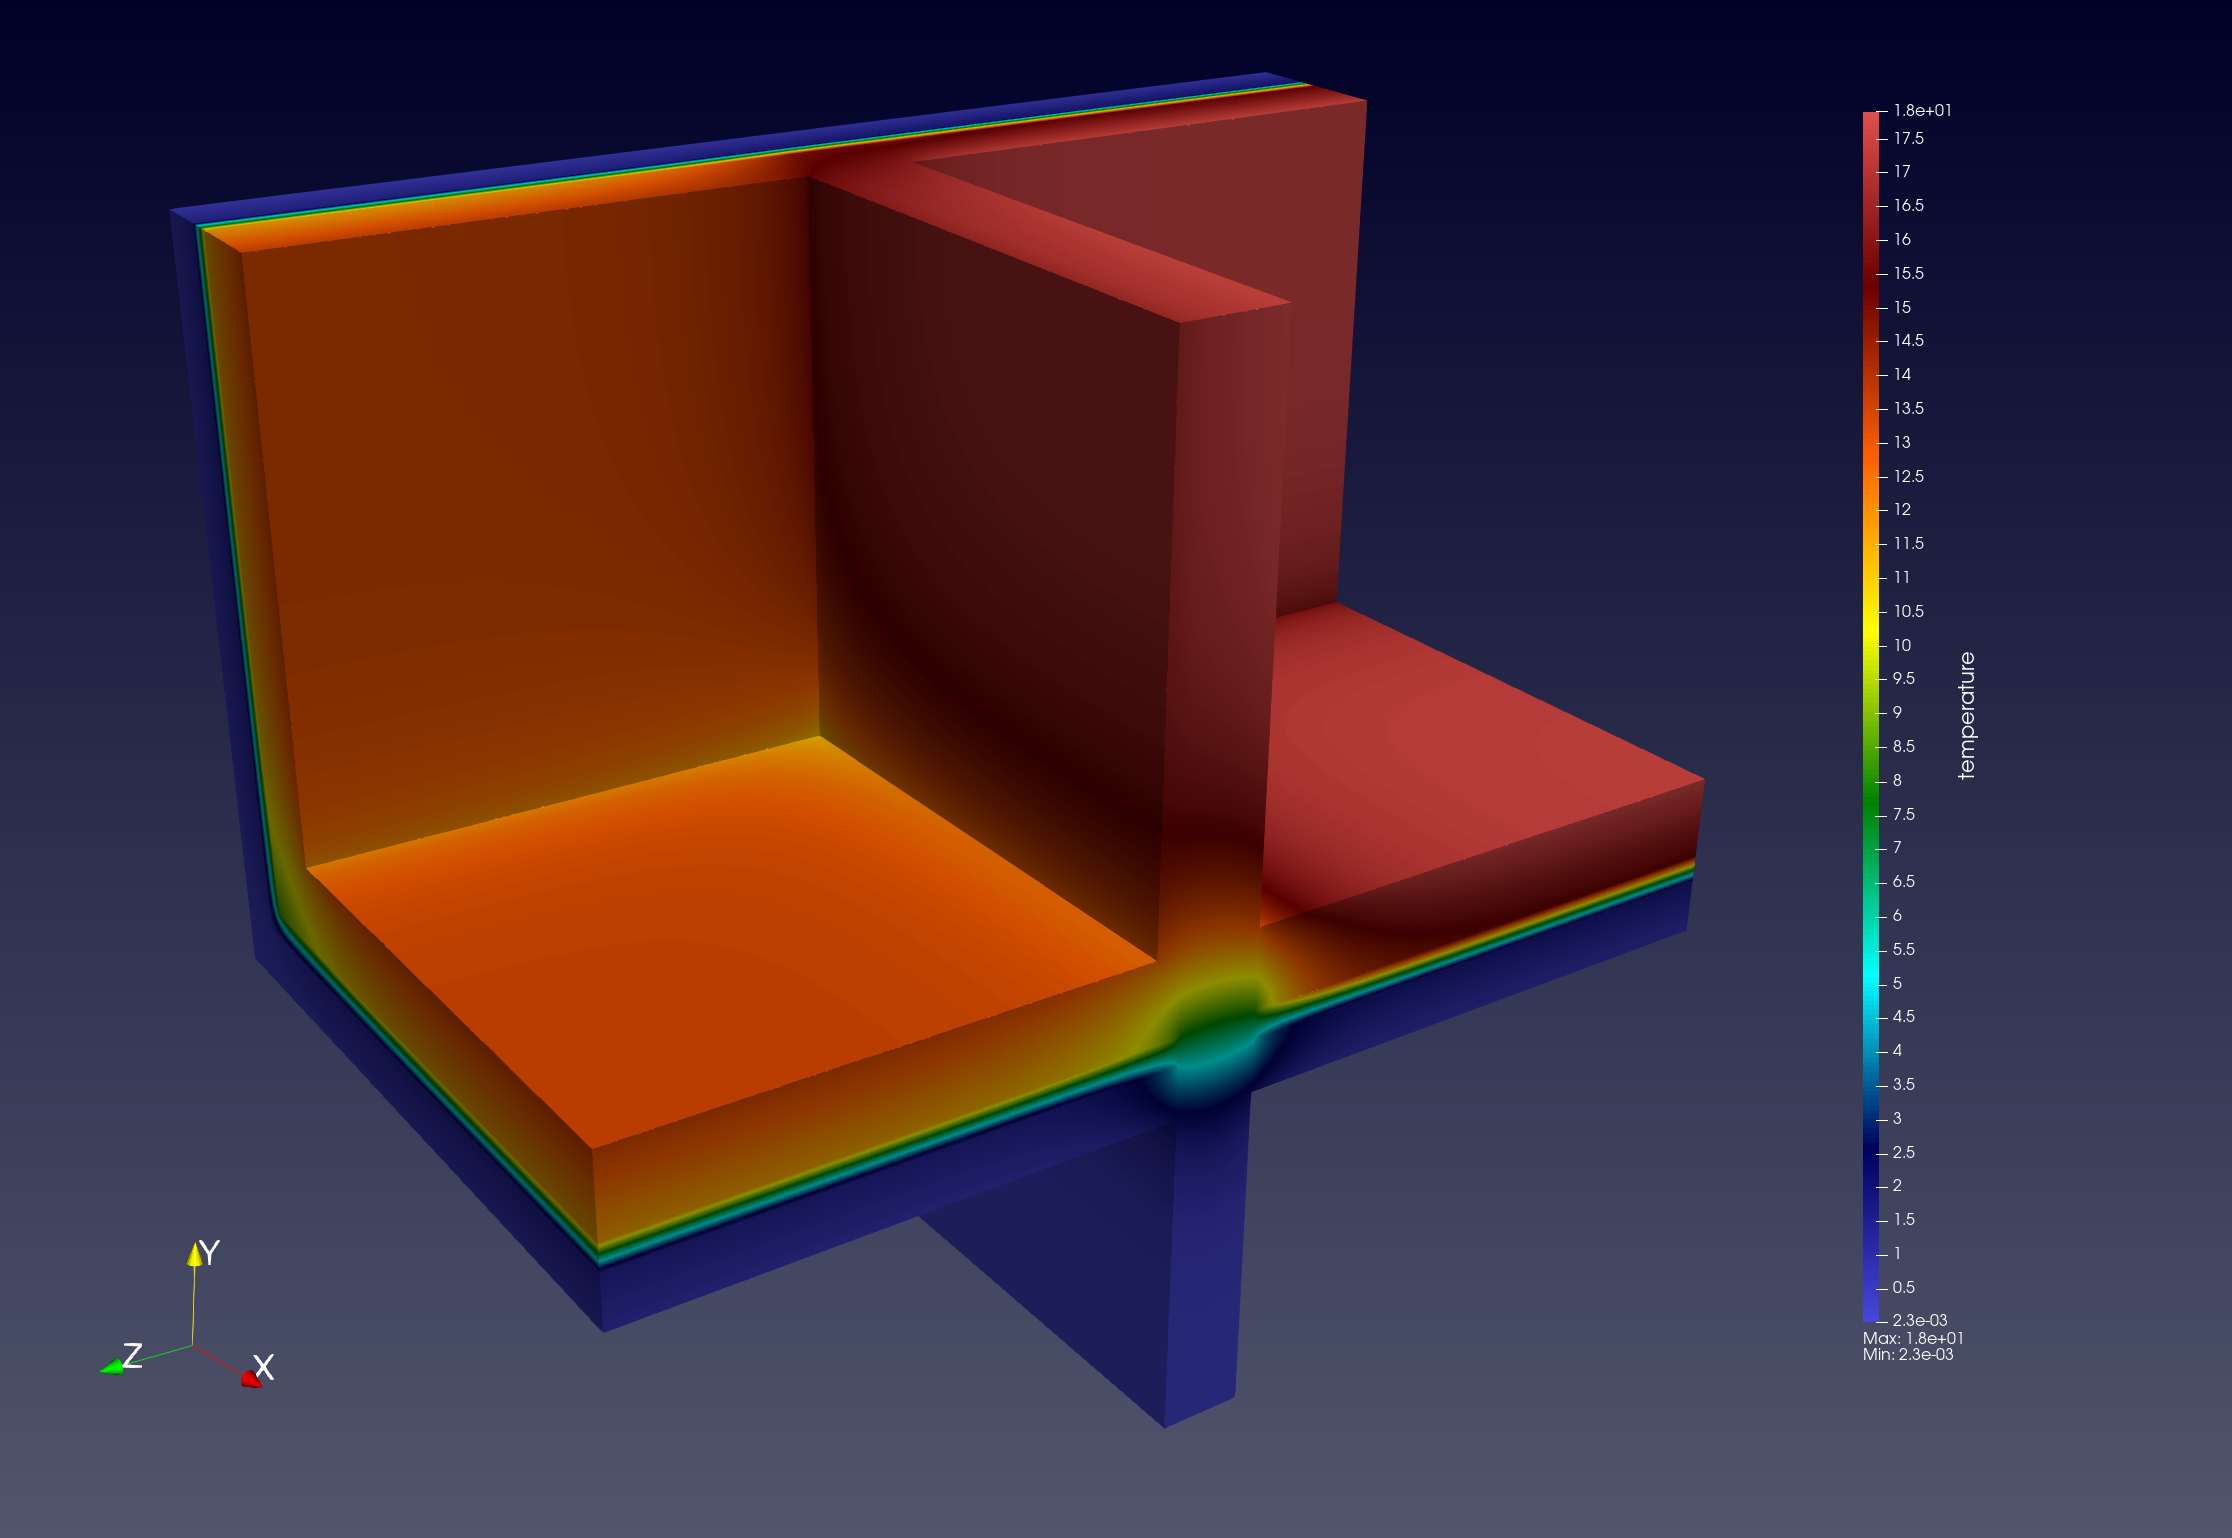
\includegraphics[width=\textwidth]{graphics/feelpp/feelpp-benchmark-thermalbridges-solution.png}
  \end{subfigure}
  \hfill
  \begin{subfigure}[c]{0.49\textwidth}
    \centering
    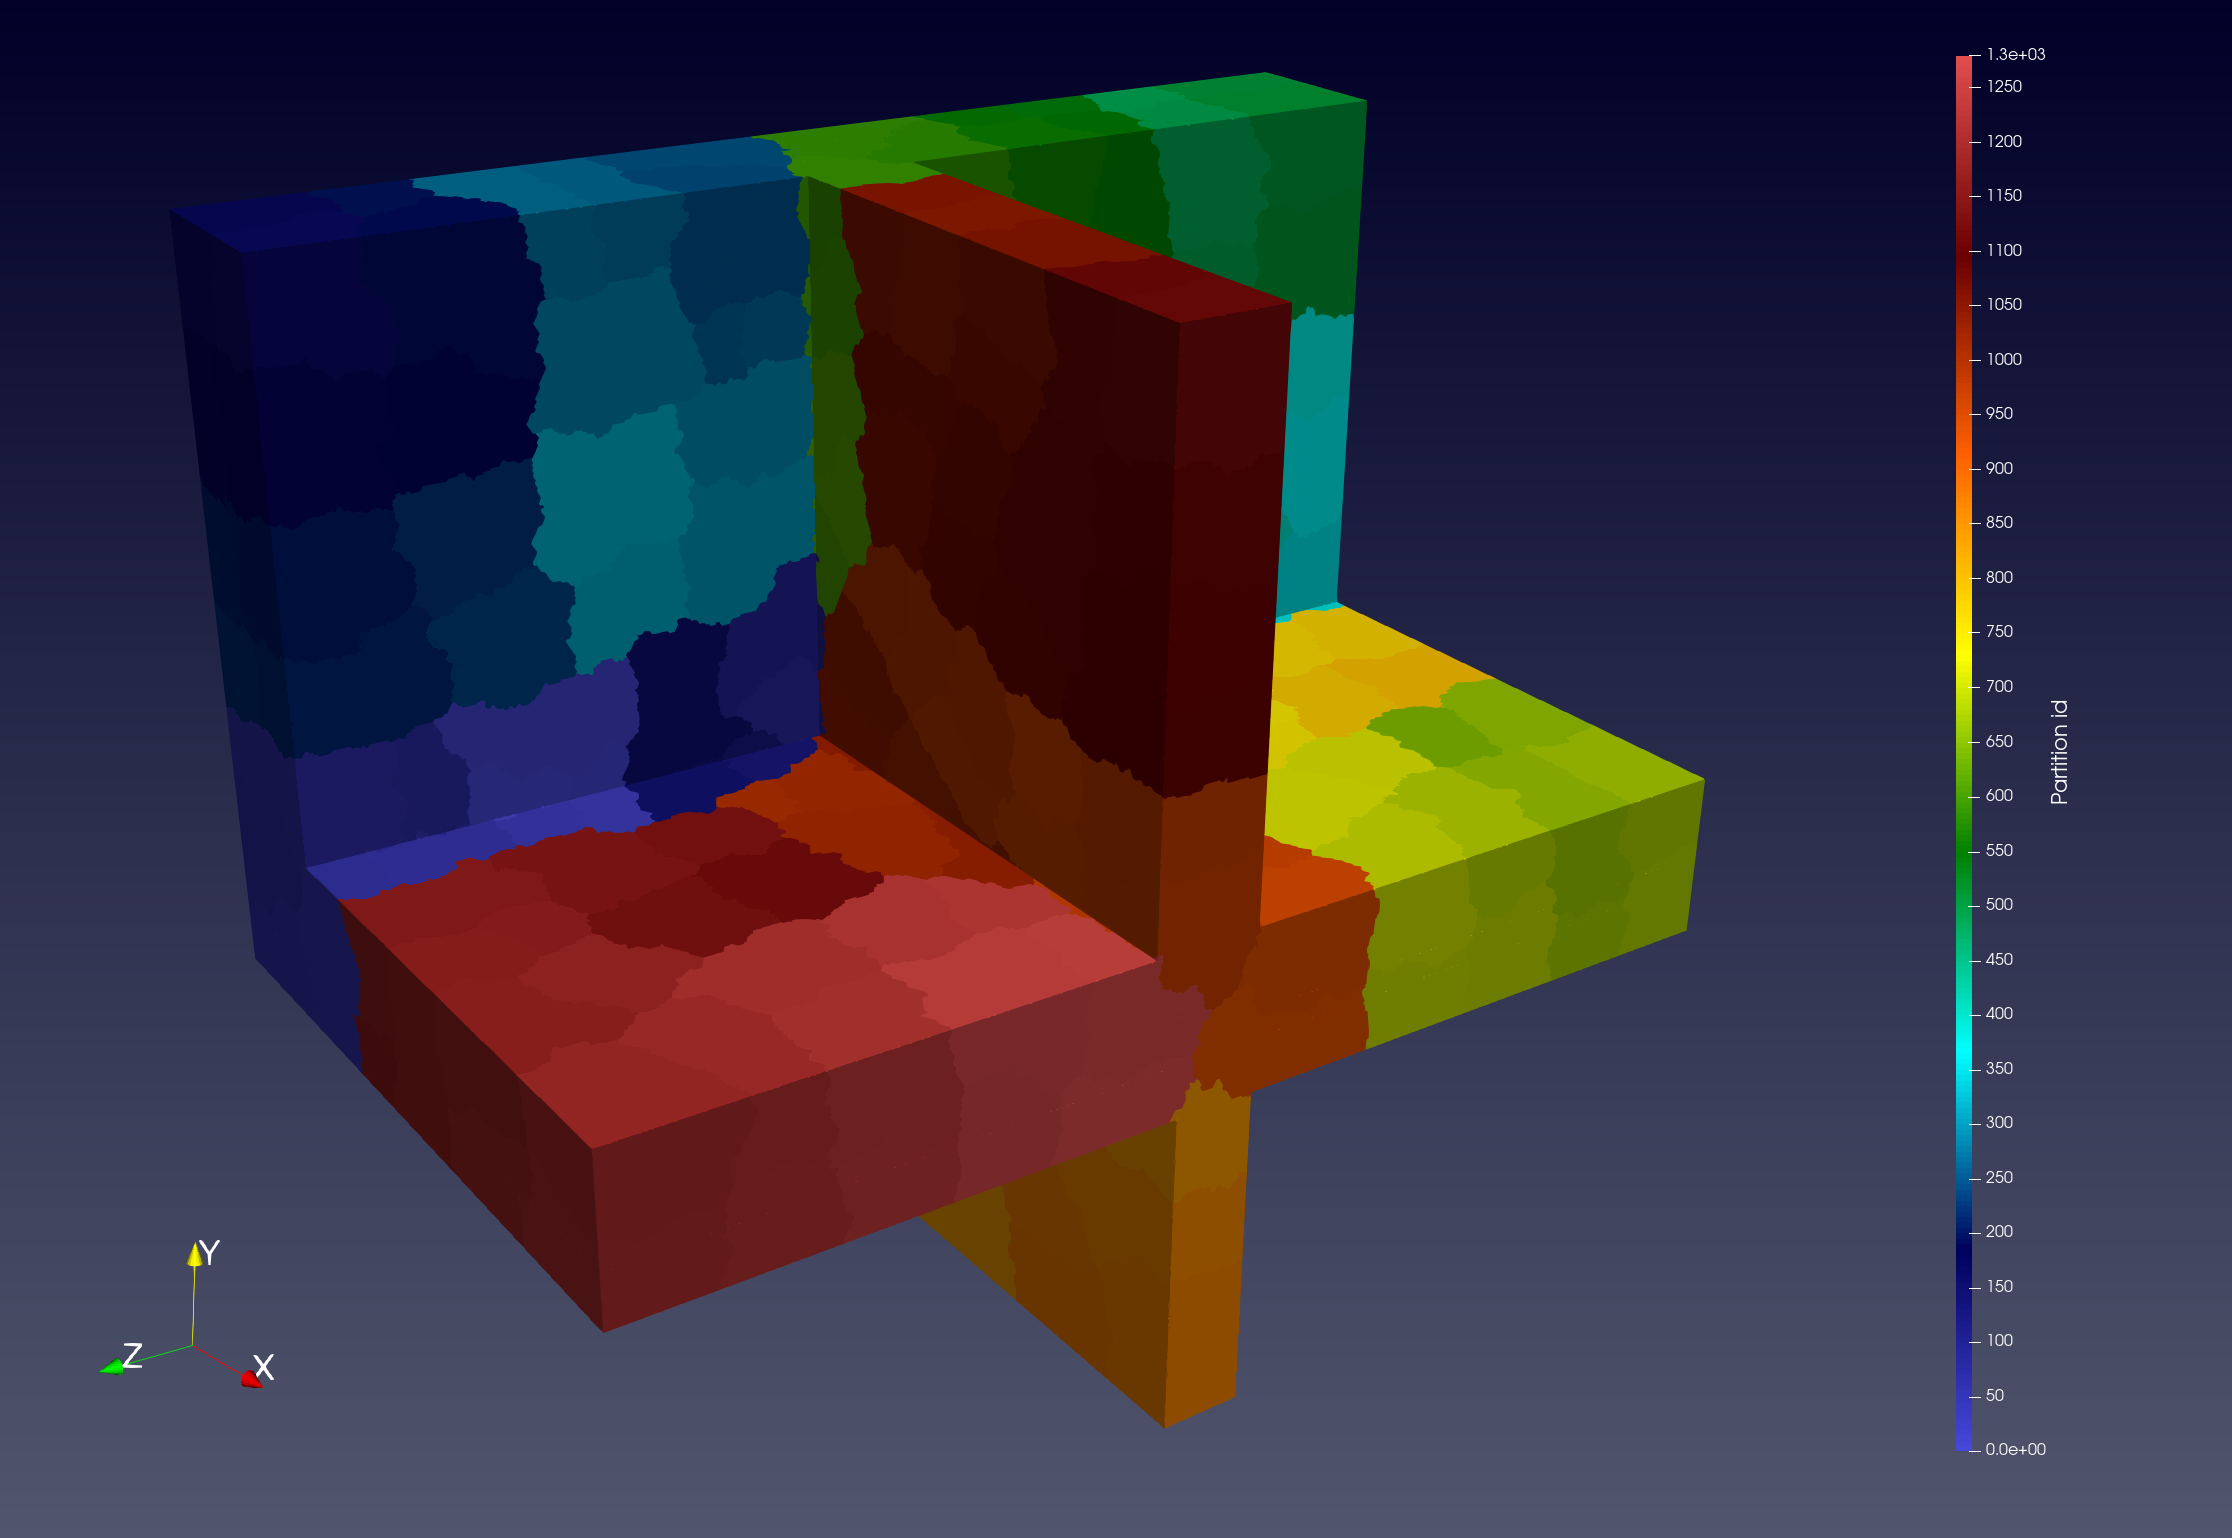
\includegraphics[width=\textwidth]{graphics/feelpp/feelpp-benchmark-thermalbridges-pid.png}
  \end{subfigure}
  \caption{Thermal bridges benchmarks - temperature solution (left) and
    partitioning example (right)}
  \label{fig:wp1:feelpp:thermal_bridges:visualization}
\end{figure}



\paragraph{Benchmarking Tools Used}

The benchmark was performed on the \textbf{Discoverer} supercomputer (see
\Cref{sec:arch:eurohpc-ju}).
The performance tools integrated into the \Feelpp-toolboxes framework were used to measure
the execution time.
Moreover, we need to note that we have used here Apptainer with \Feelpp SIF image based on Ubuntu noble OS.

The metrics measured are the execution time of the main components of the simulation. We enumerate these parts in the following:
\begin{itemize}
\item \textbf{Init}: load mesh from filesystem and initialize heat toolbox (finite element context and algebraic data structure)
\item \textbf{Assembly}: calculate and assemble the matrix and rhs values obtained using the finite element method
\item \textbf{Solve}: the linear system by using a preconditioned gmres
\item \textbf{PostProcess}: compute validation measures (temperature at points and
  heat flux) and export on the filesystem a visualization format (EnsighGold) of
  the solution.
\end{itemize}

\paragraph{Input/Output Dataset Description}

\begin{itemize}
\item \textbf{Input Data:}
  \begin{itemize}
  \item Meshes: We have generated three levels of mesh called M1, M2
    and M3. These meshes are stored in GMSH format. The statistics can be found in
    \Cref{tab:wp1:feelpp:thermal_bridges:discr_stat}. We have also prepared for
    each mesh level a collection of partitioned mesh.
    The format used is an in-house mesh format of \Feelpp based on
    JSON+HDF5 file type.
    The Gmsh meshes and the partitioned meshes can be found on our Girder
    database management, in the \Feelpp collections.
  \item Setup: Use standard setup of \Feelpp toolboxes. It corresponds to a cfg
    file and JSON file. These config files are present in the Github of feelpp.
  \item Sif image: feelpp:v0.111.0-preview.10-noble-sif  (stored in the Github registry of \Feelpp)
  \end{itemize}
\item \textbf{Output Data:} The output includes the computed values of
  validation measure in CSV files format, export visualization files (mesh, partitioning, temperature), and the time taken to perform each simulation step.
\end{itemize}



\begin{table}[h!]
  \centering
  { \setlength{\parindent}{0pt}
    \def\arraystretch{1.25}
    \arrayrulecolor{numpexgray}
    {\fontsize{9}{11}\selectfont
      \begin{tabular}{!{\color{numpexgray}\vrule}c!{\color{numpexgray}\vrule}c!{\color{numpexgray}\vrule}c!{\color{numpexgray}\vrule}c!{\color{numpexgray}\vrule}c!{\color{numpexgray}\vrule}c!{\color{numpexgray}\vrule}c!{\color{numpexgray}\vrule}c!{\color{numpexgray}\vrule}}
        \rowcolor{numpexgray}\multicolumn{5}{c!{\color{numpexgray}\vrule}}{\color{white}\bf Mesh properties}
        & \multicolumn{3}{c!{\color{numpexgray}\vrule}}{\color{white}\bf Number of degrees of freedom} \\
        \rowcolor{numpexgray} {\color{white}\bf Tag} & {\color{white}\bf \# points} & {\color{white}\bf \# edges} & {\color{white}\bf \# faces} & {\color{white}\bf \# elements} & {\color{white}\bf $P_1$} & {\color{white}\bf $P_2$} & {\color{white}\bf $P_3$} \\
        \texttt{M1} & \pgfmathprintnumber{193654} & \pgfmathprintnumber{1299920} & \pgfmathprintnumber{2164759} & \pgfmathprintnumber{1058492} & \pgfmathprintnumber{193654} & \pgfmathprintnumber{1493574} & \pgfmathprintnumber{4958253} \\
        \texttt{M2} & \pgfmathprintnumber{1401135} & \pgfmathprintnumber{9778744} & \pgfmathprintnumber{16566803} & \pgfmathprintnumber{8189193} & \pgfmathprintnumber{1401135} & \pgfmathprintnumber{11179879} & \pgfmathprintnumber{37525426} \\
        \texttt{M3} & \pgfmathprintnumber{10572256} & \pgfmathprintnumber{75307308} & \pgfmathprintnumber{128722252} & \pgfmathprintnumber{63987199} & \pgfmathprintnumber{10572256} & \pgfmathprintnumber{85879564} & \pgfmathprintnumber{289909124} \\
        \hline
      \end{tabular}
    }}
  \caption{Thermal bridges benchmarks - Statistics on meshes and number of degrees of freedom with respect
    to finite element approximation}
  \label{tab:wp1:feelpp:thermal_bridges:discr_stat}
\end{table}


\paragraph{Results Summary}
The benchmark results are summarized in
\Cref{fig:feelpp:wp1:thermal_bridges:performance_times_M1},
\Cref{fig:feelpp:wp1:thermal_bridges:performance_times_M2},
\Cref{fig:feelpp:wp1:thermal_bridges:performance_times_M3} which correspond respectively to
choice of the mesh M1, M2 and M3. Moreover, for each mesh, we have experimented with several
finite element discretizations called $P_1$, $P_2$ and $P_3$.
For each order of finite element approximation, we have selected a set of number
of CPU cores.

Firstly, we can see clearly that the Solve part is the most time-consuming. See
comments in \Cref{sec:WP3:Feelpp:benchmark:thermal_bridges}.
Concerning the mesh M1, considered a coarse mesh, we note that the
scalability scaling is not good, especially for low order. This is simply because the problem is too small for so many HPC resources. MPI
communications an IO effects are non-negligible.
For the mesh M2, results are better (but not ideal) up to around one thousand processing cores.
Finally, the fined mesh M3, illustrates the best scalability on this range of
number of tasks. Except for the solve part, we can see an efficiency of increased
HPC resource at this level.

Each run illustrated here is also validated thanks to the value of the ISO 10211:2017 standard.
With these experiments, we have also seen that we have some variability in
performance measures. Some aspects like the filesystem and network load, are not
under our control, it can explain a part of this. Also, the memory and
consequently the choice of the number of tasks per node can be important and
can change significantly the performance. This latter will be taken into account
more accurately in a next campaign of these benchmarking test.

\newcommand{\barChart}[2][ybar]{
  \begin{tikzpicture}
    \begin{axis}[
      width=\textwidth, height=0.6172\textwidth,
      xlabel={Number of CPU core}, ylabel={Execution time [s]},
      %xticklabels from table={#2}{nProc},
      xtick=data,
      xtick align=outside,
      ymin=0,
      %legend style={at={(1,1)}, anchor=north east},
      %legend style={at={(0.5,1)}, anchor=south,font=\tiny,legend columns=-1},
      ymajorgrids=true, yminorgrids=true,
      bar width=7pt,
      #1
    ]
    \foreach [expand list=true] \thetuple in {#2} {
      \pgfkeys{/mysettings/.cd,
        table/.store in=\mytable,
        column/.store in=\mycolumn,
        shift/.store in=\myshift, shift/.default=0, shift,
        legend/.store in=\mylegend,
        color/.store in=\mycolor
      }
      \edef\temp{
        \noexpand\pgfkeys{/mysettings/.cd, \expandafter\@firstofone\thetuple}
      } \temp
      %\def\toto{\expandafter\mytable}
      \edef\temp{
        \noexpand\addplot[ybar, bar width=0.2, fill=\mycolor, draw=black, point meta=y]
        table [x expr=\noexpand\coordindex+\myshift, y=\mycolumn ] {\expandafter\noexpand\csname \mytable\endcsname};
        %table [x=nProc, y=\mycolumn ] {\expandafter\noexpand\csname \mytable\endcsname};
      } \temp
      %table [x expr=\noexpand\coordindex, y=\mycolumn ] {#2};
      \edef\temp{
        \noexpand\addlegendentry{\mylegend}
      } \temp
    }
    \end{axis}
\end{tikzpicture}
}


\foreach [expand list=true] \meshId in {1,2,3} {

  \pgfplotstableread[col sep=comma]{\currfiledir/data/thermalbridges_M\meshId_P1_discoverer.csv}\dataPa
  \pgfplotstableread[col sep=comma]{\currfiledir/data/thermalbridges_M\meshId_P2_discoverer.csv}\dataPb
  \pgfplotstableread[col sep=comma]{\currfiledir/data/thermalbridges_M\meshId_P3_discoverer.csv}\dataPc

  \begin{figure}
    \centering
    \def\plotSetup##1{
      {table=##1,column=init,legend=Init,color=customdarkblue},
      {table=##1,legend=Assembly,column=algebraic-assembly,color=customcyan},
      {table=##1,legend=Solve,column=algebraic-solve,color=customorange},
      {table=##1,legend=PostProcess,column=exportResults,color=custompurple}
    }
    \def\chartBarPlot##1##2{
      \barChart[ybar,
      xticklabels from table={##2}{nProc},
      legend style={at={(0.5,1)}, anchor=south,font=\tiny,legend columns=-1}
      ]{\plotSetup{##1}}
    }
    \def\chartBarStackedPlot##1##2{
      \barChart[ybar stacked,
      xticklabels from table={##2}{nProc},
      legend style={at={(0.5,1)}, anchor=south,font=\tiny,legend columns=-1}
      ]{\plotSetup{##1}}
    }

    \begin{subfigure}[c]{0.49\textwidth}
      \centering
      \chartBarPlot{dataPa}{\dataPa}
      \caption{\texttt{M\meshId} - \texttt{$P_1$}}
    \end{subfigure}
    \hfill
    \begin{subfigure}[c]{0.49\textwidth}
      \centering
      \chartBarStackedPlot{dataPa}{\dataPa}
      \caption{\texttt{M\meshId} - \texttt{$P_1$}}
    \end{subfigure}
    \hfill
    \begin{subfigure}[c]{0.49\textwidth}
      \centering
      \chartBarPlot{dataPb}{\dataPb}
      \caption{\texttt{M\meshId} - \texttt{$P_2$}}
    \end{subfigure}
    \hfill
    \begin{subfigure}[c]{0.49\textwidth}
      \centering
      \chartBarStackedPlot{dataPb}{\dataPb}
      \caption{\texttt{M\meshId} - \texttt{$P_2$}}
    \end{subfigure}
    \hfill
    \begin{subfigure}[c]{0.49\textwidth}
      \centering
      \chartBarPlot{dataPc}{\dataPc}
      \caption{\texttt{M\meshId} - \texttt{$P_3$}}
    \end{subfigure}
    \hfill
    \begin{subfigure}[c]{0.49\textwidth}
      \centering
      \chartBarStackedPlot{dataPc}{\dataPc}
      \caption{\texttt{M\meshId} - \texttt{$P_3$}}
    \end{subfigure}
    \caption{Thermal bridges benchmarks - Execution time of main simulation components
      - Mesh \texttt{M\meshId} - Discoverer supercomputer}
    \label{fig:feelpp:wp1:thermal_bridges:performance_times_M\meshId}
  \end{figure}

}




% columns/FunctionSpace/.style={string type},
\begin{figure}
  \centering
  \captionsetup[subfigure]{justification=centering}

  \pgfplotstableread[col sep=comma]{\currfiledir/data/measures_all.csv}\dataTableMeasures
  \def\myLineWidth{2pt}
  \def\myLineStyleA{loosely dashdotdotted} %dashdotdotted
  \def\myLineStyleB{dashed}
  \def\myLineStyleC{solid}

  \def\myAddPlot#1#2#3#4{
    \addplot[#3,every mark/.append style={solid},
    % x filter/.expression={(\thisrow{PolyOrder} == 1 ?  \pgfmathparse{\thisrow{Mesh}}\pgfmathresult :NaN)},
    % x filter/.expression={ \thisrow{FunctionSpace} == \thisrow{FunctionSpace} ? \pgfmathresult
    % x filter/.expression={(\thisrow{FunctionSpace} == P1 ? \pgfmathresult :NaN )},
    x filter/.code={
      \pgfmathparse{\thisrow{PolyOrder}==#2}
      \ifnum0=\pgfmathresult
      \pgfmathsetmacro{\newx}{nan}
    \else
      \pgfmathsetmacro{\newx}{\thisrow{Mesh}}
    \fi
    \pgfmathparse{\newx}
  },
  y filter/.expression={ #4*\pgfmathresult }
  ] table [x=Mesh, y=#1] {\dataTableMeasures};
  }

  \def\myPlotOutputMeasures#1#2#3#4{
      \resizebox{\textwidth}{0.6172\textwidth}{
    \begin{tikzpicture}
    \begin{axis}[
      %width=\textwidth, height=1.2\textheight,
      xtick=data,
      xticklabel={M$\pgfmathprintnumber{\tick}$},
      xmajorgrids=true,% xminorgrids=false, minor x tick num=3,
      ymajorgrids=true, yminorgrids=true,
      minor y tick num=2,
      % xticklabel={\pgfmathparse{100*\tick}\pgfmathprintnumber[precision=0]{\pgfmathresult}\%},
      %xticklabel={\pgfmathparse{\tick}\pgfmathprintnumber[fixed,set thousands separator={},precision=0]{\pgfmathresult}},
      xlabel={Mesh levels}, ylabel={#4},
      % legend style={at={(0.5,1)}, anchor=south,font=\small,legend columns=3}
      %legend style={at={(0.,1)}, anchor=north west,font=\small,legend
      %columns=3},
      legend style={at={(0.,1)}, anchor=south west,font=\small,legend columns=4},
      %#2
      ]

      \myAddPlot{#1}{1}{color=customdarkblue,\myLineStyleC,mark=o,line width=\myLineWidth}{#2}
      \addlegendentry{P1}
      \myAddPlot{#1}{2}{color=customcyan,\myLineStyleC,mark=triangle,line width=\myLineWidth}{#2}
      \addlegendentry{P2}
      \myAddPlot{#1}{3}{color=customorange,\myLineStyleC,mark=square,line width=\myLineWidth}{#2}
      \addlegendentry{P3}
      \addplot+[color=red,\myLineStyleB,mark=none,line width=\myLineWidth,every mark/.append style={solid}] coordinates {
        (1,#3) (3,#3)
      };
      \addlegendentry{Ref}

    \end{axis}
  \end{tikzpicture}
      }

}

  \begin{subfigure}[c]{0.49\textwidth}
    \centering
    \myPlotOutputMeasures{Normal_Heat_Flux_alpha}{1}{46.09}{Heat flow [W]}
    \caption{Heat flow measured in $\alpha$ environment}
  \end{subfigure}
  \hfill
  \begin{subfigure}[c]{0.49\textwidth}
    \centering
    \myPlotOutputMeasures{Normal_Heat_Flux_beta}{1}{13.89}{Heat flow [W]}
    \caption{Heat flow measured in $\beta$ environment}
  \end{subfigure}
  \hfill
  \begin{subfigure}[c]{0.49\textwidth}
    \centering
    \vspace*{0.03\textheight}
    \myPlotOutputMeasures{Normal_Heat_Flux_gamma}{-1}{59.98}{Heat flow [W]} % warning inverse
    \caption{Heat flow measured in $\gamma$ environment}
  \end{subfigure}
  \hfill
  \begin{subfigure}[c]{0.49\textwidth}
    \centering
    \vspace*{0.03\textheight}
    \myPlotOutputMeasures{Statistics_temperature_alpha_min}{1}{11.32}{Temperature
      [°C]}
    \caption{Surface temperature min in $\alpha$ environment}
  \end{subfigure}

  \caption{Thermal bridges benchmarks - Convergence of validation measures compared to references values}
    \label{fig:feelpp:wp1:thermal_bridges:measures_convergences}
\end{figure}



\paragraph{Challenges Identified}
Several challenges were encountered during the benchmarking process:
\begin{itemize}
    \item \textbf{Memory Usage:} We need to check and detect the memory
      consumed during the simulation to avoid bad behavior like swapping.
    \item \textbf{Parallelization Inefficiencies:} We need to understand and
      improve performance when MPI communication and filesystem IO will be dominant.
    %\item \textbf{Cache and Memory Bottlenecks:}
\end{itemize}

To conclude, we have realized HPC performance tests of benchmark called thermal
bridges. We have realized with success the execution of several simulations on
significant resources and demonstrated the validation of \Feelpp framework in the
elliptic PDE context. We have also validated the deployment of \Feelpp with
container support. Now, we need to provide more refined measures to detect and
analyze reasons for performance degradation. And also compare to other software
installations, like Spack.





\subsubsection{Benchmark \#2: Assemble Stiffness and Linear Elasticity Matrix}

\paragraph{Description}
This benchmark evaluates the assembly of stiffness and linear elasticity finite element matrices in three dimensions using both continuous Galerkin (cG) and hybrid discontinuous Galerkin (hdG) methods using the \Feelpp toolboxes.
The problem size consists of a mesh with tetrahedral elements, executed entirely on multi-core CPU architectures.
The benchmark is designed to measure scalability, execution time, and computational efficiency across different material models, including isotropic and anisotropic materials.

The objective of the benchmark is to assess performance in terms of assembly time, memory usage, and parallel efficiency for cG and hdG methods from low to high orders using CPU resources only.

\paragraph{Benchmarking Tools Used}
The following performance analysis tools were used:
\begin{itemize}
    \item \textbf{\Feelpp}: the performance tools integrated into the \Feelpp framework were used to measure the execution time and memory usage during the matrix assembly.
\end{itemize}

Metrics such as execution time, memory usage, and FLOPS were measured to compare the performance of the cG and hdG methods on CPU.

\paragraph{Input/Output Dataset Description}
\begin{itemize}
    \item \textbf{Input Data:} The input dataset consists of a 3D tetrahedral mesh generated using the Gmsh format, with approximately 1 million elements. Material properties are defined in JSON format, covering both isotropic and anisotropic materials.

    \item \textbf{Output Data:} The output includes performance logs, execution times, and memory usage reports. Output results are replicable by using the same mesh and material properties.

    \item \textbf{Data Repository:} All input and output datasets are available in a Zenodo repository, accessible through DOI: \texttt{[Insert DOI]}.
\end{itemize}


\begin{table}[h!]
  \centering
  { \setlength{\parindent}{0pt}
    \def\arraystretch{1.25}
    \arrayrulecolor{numpexgray}
    {\fontsize{9}{11}\selectfont
      \begin{tabular}{!{\color{numpexgray}\vrule}c!{\color{numpexgray}\vrule}c!{\color{numpexgray}\vrule}c!{\color{numpexgray}\vrule}c!{\color{numpexgray}\vrule}c!{\color{numpexgray}\vrule}c!{\color{numpexgray}\vrule}c!{\color{numpexgray}\vrule}c!{\color{numpexgray}\vrule}}
        \rowcolor{numpexgray}\multicolumn{5}{c!{\color{numpexgray}\vrule}}{\color{white}\bf Mesh properties}
        & \multicolumn{2}{c!{\color{numpexgray}\vrule}}{\color{white}\bf Number of degrees of freedom} \\
        \rowcolor{numpexgray} {\color{white}\bf Tag} & {\color{white}\bf \# points} & {\color{white}\bf \# edges} & {\color{white}\bf \# faces} & {\color{white}\bf \# elements} & {\color{white}\bf $P_1$} & {\color{white}\bf $P_2$} \\
        \texttt{M2} & \pgfmathprintnumber{324257} & \pgfmathprintnumber{2247489} & \pgfmathprintnumber{3796235} & \pgfmathprintnumber{1873002} & \pgfmathprintnumber{972771} & \pgfmathprintnumber{7715238}  \\
        \texttt{M3} & \pgfmathprintnumber{2426377} & \pgfmathprintnumber{17230019} & \pgfmathprintnumber{29409215} & \pgfmathprintnumber{14605572} & \pgfmathprintnumber{7279131} & \pgfmathprintnumber{58969188}  \\
        \texttt{M4} & \pgfmathprintnumber{18801264} & \pgfmathprintnumber{135213828} & \pgfmathprintnumber{232036941} & \pgfmathprintnumber{115624376} & \pgfmathprintnumber{56403792} & \pgfmathprintnumber{462045276} \\
        \hline
      \end{tabular}
    }}
  \caption{NAFEMS le10 benchmark - Statistics on meshes and number of degrees of freedom with respect
    to finite element approximation}
  \label{tab:wp1:feelpp:thermal_bridges:discr_stat}
\end{table}


\paragraph{Results Summary}
The benchmark results are summarized as follows:

RESULTS here

The results highlight that ... (ADD ANALYSIS)


\foreach [expand list=true] \meshId in {2,3,4} {

  \pgfplotstableread[col sep=comma]{\currfiledir/data/nafems_le10_M\meshId_P1_discoverer.csv}\dataPa
  \pgfplotstableread[col sep=comma]{\currfiledir/data/nafems_le10_M\meshId_P2_discoverer.csv}\dataPb

  \begin{figure}
    \centering
    \def\plotSetup##1{
      {table=##1,column=init,legend=Init,color=customdarkblue},
      {table=##1,legend=Assembly,column=algebraic-assembly,color=customcyan},
      %{table=##1,legend=Solve,column=algebraic-solve,color=customorange},
      {table=##1,legend=PostProcess,column=exportResults,color=custompurple}
    }
    \def\chartBarPlot##1##2##3{
      \barChart[ybar,xticklabels from table={##2}{nProc},legend style={at={(0.5,1)}, anchor=south,font=\tiny,legend columns=-1},##3]{\plotSetup{##1}}
    }
    \def\chartBarStackedPlot##1##2{
      \barChart[ybar stacked,xticklabels from table={##2}{nProc},
      legend style={at={(0.5,1)}, anchor=south,font=\tiny,legend columns=-1}
      ]{\plotSetup{##1}}
    }

    \begin{subfigure}[c]{0.49\textwidth}
      \centering
      \chartBarPlot{dataPa}{\dataPa}{}
      \caption{\texttt{M\meshId} - \texttt{$P_1$}}
    \end{subfigure}
    \hfill
    \begin{subfigure}[c]{0.49\textwidth}
      \centering
      \chartBarStackedPlot{dataPa}{\dataPa}
      \caption{\texttt{M\meshId} - \texttt{$P_1$}}
    \end{subfigure}
    \hfill
    \begin{subfigure}[c]{0.49\textwidth}
      \centering
      \ifnum4=\meshId
      \chartBarPlot{dataPb}{\dataPb}{enlarge x limits=0.3}
    \else
      \chartBarPlot{dataPb}{\dataPb}{}
    \fi



      \caption{\texttt{M\meshId} - \texttt{$P_2$}}
    \end{subfigure}
    \hfill
    \begin{subfigure}[c]{0.49\textwidth}
      \centering
      \chartBarStackedPlot{dataPb}{\dataPb}
      \caption{\texttt{M\meshId} - \texttt{$P_2$}}
    \end{subfigure}
    \caption{NAFEMS le10 benchmarks - Execution time of main simulation components
      - Mesh \texttt{M\meshId} - Discoverer supercomputer}
    \label{fig:feelpp:wp1:nafems_le10:performance_times_M\meshId}
  \end{figure}

}



\paragraph{Challenges Identified}
Several challenges were encountered during the benchmarking process:
\begin{itemize}
    \item \textbf{Memory Usage:}
    \item \textbf{Parallelization Inefficiencies:}
    \item \textbf{Cache and Memory Bottlenecks:}
\end{itemize}

add extra analysis  and conclusion here.

\subsubsection{Benchmark \#3: Thermo-Electric Coupling}

Thermo Electric coupling in a complex geometry.








\subsubsection{Benchmark \#4: HeatFluid Coupling}
\label{sec:WP1:Feelpp:benchmark4}

\newcommand{\vct}[1]{\vec{#1}}
\newcommand{\mat}[1]{\underline{\underline{#1}}}


% \emph{enlever tous les détails, et laisser les références, expliciter la liste de maillage et la machine où est faite le bench, et la mise en donnée (paramètrisation)}

% \emph{dans wp3: parler du préconditionner}


\paragraph{Description}
This benchmark models the steady aqueous humor (AH) flow in the posterior and anterior chambers of the human eyeball, coupled with the overall heat transfer, adapted from~\cite{ooi_simulation_2008,kilgour_operator_2021}.
The full model description is available in~\cite{saigre_coupled_2024_abstract}.
It it run with the toolbox \texttt{heatfluid} of \Feelpp.


\paragraph{Benchmarking Tools Used}

The following tools were used for performance profiling and analysis:
\begin{itemize}
    \item \textbf{\Feelpp}: the performance tools integrated into the \Feelpp framework were used to measure the execution time.
    \item \textbf{Gaya}: the benchmark was performed on the Gaya supercomputer (see \Cref{sec:arch:gaya}).
\end{itemize}

The metrics measured are the execution time to:
\begin{inparaenum}[\it (i)]
    \item load and initialize the mesh that is already partitioned on the disk,
    \item initialize the data structures,
    \item assembly algebraic objects of the linear system,
    \item solve the non-linear algebraic system, and
    \item export the results.
\end{inparaenum}


\paragraph{Input/Output Dataset Description}

\begin{itemize}
    \item \textbf{Input Data:} The input dataset consists of a family of 3D tetrahedral meshes generated through the process described in~\cite{chabannes_3d_2024}, and denoted \texttt{Mr0} to \texttt{Mr6}, with an increasing number of elements.
    \Cref{tab:feelpp:wp1:coupled:mesh} presents the characteristics of these meshes.
    The input data also provides the configuration files necessary to run the simulations.
    \item \textbf{Output Data:} The output includes the computed temperature, velocity, and pressure fields for each mesh, stored in HDF5 format, as well as the time taken to perform each step of the simulation.
    \item \textbf{Data Repository:} All input and output datasets are available in a Zenodo repository \cite{saigre_mesh_2024}, accessible through DOI: \href{https://doi.org/10.5281/ZENODO.13886143}{10.5281/ZENODO.13886143}.
\end{itemize}


\begin{table}[!ht]
    \centering
    { \setlength{\parindent}{0pt}
    \def\arraystretch{1.25}
    \arrayrulecolor{numpexgray}
    {\fontsize{9}{11}\selectfont
    \begin{tabular}{!{\color{numpexgray}\vrule}c!{\color{numpexgray}\vrule}c!{\color{numpexgray}\vrule}c!{\color{numpexgray}\vrule}c!{\color{numpexgray}\vrule}c!{\color{numpexgray}\vrule}c!{\color{numpexgray}\vrule}c!{\color{numpexgray}\vrule}c!{\color{numpexgray}\vrule}}
        \rowcolor{numpexgray}
        \multicolumn{5}{c!{\color{numpexgray}\vrule}}{\color{white}\bf Mesh properties} & \multicolumn{3}{c!{\color{numpexgray}\vrule}}{\color{white}\bf Number of degrees of freedom} \\
        \hline
        \rowcolor{numpexgray}{\color{white}\bf Tag} & {\color{white}\bf $h_\text{min}$} & {\color{white}\bf $h_\text{max}$} & {\color{white}\bf $h_\text{mean}$} & {\color{white}\bf \# elements} & {\color{white}\bf $T$} & {\color{white}\bf $\vct{u}$} & {\color{white}\bf $p$} \\
        \texttt{Mr0} & \pgfmathprintnumber{1.247583e-04} & \pgfmathprintnumber{3.997611e-03} & \pgfmathprintnumber{9.227331e-04} & \pgfmathprintnumber{191939} & \pgfmathprintnumber{37470} & \pgfmathprintnumber{84966} & \pgfmathprintnumber{4615} \\
        \rowcolor{numpexlightergray}
        \texttt{Mr1} & \pgfmathprintnumber{1.367312e-04} & \pgfmathprintnumber{3.634717e-03} & \pgfmathprintnumber{7.717604e-04} & \pgfmathprintnumber{282030} & \pgfmathprintnumber{51753} & \pgfmathprintnumber{116709} & \pgfmathprintnumber{6155} \\
        \texttt{Mr2} & \pgfmathprintnumber{6.539683e-05} & \pgfmathprintnumber{1.599067e-03} & \pgfmathprintnumber{4.668270e-04} & \pgfmathprintnumber{746664} & \pgfmathprintnumber{131327} & \pgfmathprintnumber{589992} & \pgfmathprintnumber{28548} \\
        \rowcolor{numpexlightergray}
        \texttt{Mr3} & \pgfmathprintnumber{3.294835e-05} & \pgfmathprintnumber{9.592658e-04} & \pgfmathprintnumber{4.166619e-04} & \pgfmathprintnumber{1403433} & \pgfmathprintnumber{241831} & \pgfmathprintnumber{707532} & \pgfmathprintnumber{34304} \\
        \texttt{Mr4} & \pgfmathprintnumber{2.549458e-05} & \pgfmathprintnumber{5.293352e-04} & \pgfmathprintnumber{2.883913e-04} & \pgfmathprintnumber{6038645} & \pgfmathprintnumber{1027375} & \pgfmathprintnumber{1024008} & \pgfmathprintnumber{48534} \\
        \rowcolor{numpexlightergray}
        \texttt{Mr5} & \pgfmathprintnumber{3.120124e-05} & \pgfmathprintnumber{1.501561e-04} & \pgfmathprintnumber{2.772105e-04} & \pgfmathprintnumber{43893359} & \pgfmathprintnumber{7374833} & \pgfmathprintnumber{4616967} & \pgfmathprintnumber{205342} \\
        \texttt{Mr6} & \pgfmathprintnumber{2.820610e-05} & \pgfmathprintnumber{9.940551e-07} & \pgfmathprintnumber{1.835537e-04} & \pgfmathprintnumber{150630096} & \pgfmathprintnumber{25200452} & \pgfmathprintnumber{14671089} & \pgfmathprintnumber{636943} \\
        \hline
    \end{tabular}
    }}
    \caption{Characteristics of meshes used for the convergence study and number of degrees of freedom for temperature $T$, velocity $\vct{u}$, and pressure fields $p$, with the discretization $P_1\text{--}P_2P_1$.}%
    \label{tab:feelpp:wp1:coupled:mesh}
\end{table}


\paragraph{Results Summary}

The results of the benchmark are summarized in~\Cref{fig:feelpp:wp1:coupled:time} and~\Cref{fig:feelpp:wp1:coupled:time-rel},
showing the computational time and relative computational time for each component of the simulation, respectively.
The results are presented for the three biggest meshed of the family, namely \texttt{Mr4}, \texttt{Mr5}, and \texttt{Mr6}.
Note that for \texttt{Mr6}, the simulation dit not complete on 1 node (128 cores) due to memory limitations.

We observe that the resolution of the non-linear algebraic system is the most time-consuming part of the simulation, followed by the assembly of the linear system.
Moreover, even though the relative time is globally similar when the number of cores is increased, we note a decrease in the absolute time for various components of the simulation, except for the Post process part, which involves writing the results to disk.
The assembly time remains significant compared to other parts of the simulation, with a noticeable increase in the time spent resolving the non-linear system, which forms the largest portion of the computation.
As the number of cores increases, we also observe a proportional increase in time dedicated to I/O operations, particularly in the Post process phase, due to the larger volumes of data being written to disk.

\iffalse
\pgfplotstableread{\currfiledir/data/heatfluid-time-data.dat}\data
\begin{figure}
    \centering
    \begin{tikzpicture}
        \begin{axis}[
            width=\textwidth, height=8cm,
            xlabel={Nproc}, ylabel={Computational time [s]},
            xtick={0,1,2,3,4,5,6,7,8,9,10}, xticklabels={1,2,4,8,16,32,64,128,256,512,640},
            legend style={at={(0.5,-0.15)}, anchor=north, legend columns=-1},
            ymajorgrids=true, yminorgrids=true,
            bar width=7pt, ybar stacked,
            ymode=log,
            % title={Computational time for the 3D case},
        ]
        \addplot+[ybar, bar width=0.2, fill=customdarkblue, draw=black, point meta=y] table [x=x, y=initMesh] {\data};
        \addlegendentry{Mesh}


        \addplot+[ybar, bar width=0.2, fill=customcyan, draw=black, point meta=y] table [x=x, y expr=\thisrow{init}-\thisrow{initMesh}] {\data};
        \addlegendentry{Data Structures}

        \addplot+[ybar, bar width=0.2, fill=customorange, draw=black, point meta=y] table [x=x, y=algebraic-nlsolve] {\data};
        \addlegendentry{Solve}

        \addplot+[ybar, bar width=0.2, fill=custompurple, draw=black, point meta=y] table [x=x, y expr=\thisrow{algebraic-newton-initial-guess}+\thisrow{algebraic-jacobian}+\thisrow{algebraic-residual}] {\data};
        \addlegendentry{Assembly}

        \addplot+[ybar, bar width=0.2, fill=customgreen, draw=black, point meta=y
        ] table [x=x, y=exportResults] {\data};
        \addlegendentry{Post process}

        \end{axis}
        \end{tikzpicture}
    \caption{Computational time for the coupled heat-fluid testcase, performed on Gaya with the mesh \texttt{Mr4}.}
\end{figure}

\begin{figure}
    \centering

    \begin{tikzpicture}
        \begin{axis}[
            width=\textwidth, height=8cm,
            xlabel={Nproc}, ylabel={Relative computational time [\%]},
            xtick={0,1,2,3,4,5,6,7,8,9,10}, xticklabels={1,2,4,8,16,32,64,128,256,512,640},
            legend style={at={(0.5,-0.15)}, anchor=north, legend columns=-1},
            ymajorgrids=true, yminorgrids=true,
            bar width=7pt, ybar stacked,
            ymin=0, ymax=100,
            % title={Relative computational time for the 3D case},
        ]

        % Compute the relative time for each component by dividing by the total time
        % using the correct column names from the initial plot
        \addplot+[ybar, bar width=0.2, fill=customdarkblue, draw=black, point meta=y]
            table [x=x, y expr={100*\thisrow{initMesh}/(\thisrow{initMesh} + (\thisrow{init}-\thisrow{initMesh}) + \thisrow{algebraic-nlsolve} + (\thisrow{algebraic-newton-initial-guess} + \thisrow{algebraic-jacobian} + \thisrow{algebraic-residual}) + \thisrow{exportResults})}] {\data};
        \addlegendentry{Mesh}

        \addplot+[ybar, bar width=0.2, fill=customcyan, draw=black, point meta=y]
            table [x=x, y expr={100*(\thisrow{init}-\thisrow{initMesh})/(\thisrow{initMesh} + (\thisrow{init}-\thisrow{initMesh}) + \thisrow{algebraic-nlsolve} + (\thisrow{algebraic-newton-initial-guess} + \thisrow{algebraic-jacobian} + \thisrow{algebraic-residual}) + \thisrow{exportResults})}] {\data};
        \addlegendentry{Data Structures}

        \addplot+[ybar, bar width=0.2, fill=customorange, draw=black, point meta=y]
            table [x=x, y expr={100*\thisrow{algebraic-nlsolve}/(\thisrow{initMesh} + (\thisrow{init}-\thisrow{initMesh}) + \thisrow{algebraic-nlsolve} + (\thisrow{algebraic-newton-initial-guess} + \thisrow{algebraic-jacobian} + \thisrow{algebraic-residual}) + \thisrow{exportResults})}] {\data};
        \addlegendentry{Solve}

        \addplot+[ybar, bar width=0.2, fill=custompurple, draw=black, point meta=y]
            table [x=x, y expr={100*(\thisrow{algebraic-newton-initial-guess} + \thisrow{algebraic-jacobian} + \thisrow{algebraic-residual})/(\thisrow{initMesh} + (\thisrow{init}-\thisrow{initMesh}) + \thisrow{algebraic-nlsolve} + (\thisrow{algebraic-newton-initial-guess} + \thisrow{algebraic-jacobian} + \thisrow{algebraic-residual}) + \thisrow{exportResults})}] {\data};
        \addlegendentry{Assembly}

        \addplot+[ybar, bar width=0.2, fill=customgreen, draw=black, point meta=y]
            table [x=x, y expr={100*\thisrow{exportResults}/(\thisrow{initMesh} + (\thisrow{init}-\thisrow{initMesh}) + \thisrow{algebraic-nlsolve} + (\thisrow{algebraic-newton-initial-guess} + \thisrow{algebraic-jacobian} + \thisrow{algebraic-residual}) + \thisrow{exportResults})}] {\data};
        \addlegendentry{Post process}

        \end{axis}
    \end{tikzpicture}

    \caption{Relative time spent in each component of the computation for the coupled heat-fluid testcase, performed on Gaya with the mesh \texttt{Mr4}.}
\end{figure}
\fi


\pgfplotstableread{\currfiledir/data/heatfluid-time-M4.dat}\dataMQuatre
\pgfplotstableread{\currfiledir/data/heatfluid-time-M5.dat}\dataMCinq
\pgfplotstableread{\currfiledir/data/heatfluid-time-M6.dat}\dataMSix

\begin{figure}
    \centering
    \begin{subfigure}[b]{\textwidth}
    \begin{tikzpicture}
        \begin{axis}[
            width=\textwidth, height=8cm,
            xlabel={Nproc}, ylabel={Computational time [s]},
            xtick={0,1,2,3,4,5}, xticklabels={128,256,384,512,640,768},
            legend style={at={(0.5,-0.18)}, anchor=north, legend columns=-1},
            ymajorgrids=true, yminorgrids=true, ymin=0,
            bar width=7pt, ybar stacked,
            %ymode=log,
            % title={Computational time for the 3D case},
        ]
        \addplot+[ybar, bar width=0.2, fill=customdarkblue, draw=black, point meta=y] table [x=x, y=initMesh] {\dataMQuatre};
        % \addlegendentry{Mesh}
        \addplot+[ybar, bar width=0.2, fill=customcyan, draw=black, point meta=y] table [x=x, y expr=\thisrow{init}-\thisrow{initMesh}] {\dataMQuatre};
        % \addlegendentry{Data Structures}
        \addplot+[ybar, bar width=0.2, fill=customorange, draw=black, point meta=y] table [x=x, y expr=\thisrow{algebraic-newton-initial-guess}+\thisrow{algebraic-jacobian}+\thisrow{algebraic-residual}] {\dataMQuatre};
        % \addlegendentry{Assembly}
        \addplot+[ybar, bar width=0.2, fill=custompurple, draw=black, point meta=y] table [x=x, y=algebraic-nlsolve] {\dataMQuatre};
        % \addlegendentry{Solve}
        \addplot+[ybar, bar width=0.2, fill=customgreen, draw=black, point meta=y] table [x=x, y=exportResults] {\dataMQuatre};
        % \addlegendentry{Post process}

        \resetstackedplots

        \addplot+[ybar, bar width=0.2, fill=customdarkblue, draw=black, point meta=y, forget plot] table [x=x, y=initMesh] {\dataMCinq};
        \addplot+[ybar, bar width=0.2, fill=customcyan, draw=black, point meta=y, forget plot] table [x=x, y expr=\thisrow{init}-\thisrow{initMesh}] {\dataMCinq};
        \addplot+[ybar, bar width=0.2, fill=customorange, draw=black, point meta=y, forget plot] table [x=x, y expr=\thisrow{algebraic-newton-initial-guess}+\thisrow{algebraic-jacobian}+\thisrow{algebraic-residual}] {\dataMCinq};
        \addplot+[ybar, bar width=0.2, fill=custompurple, draw=black, point meta=y, forget plot] table [x=x, y=algebraic-nlsolve] {\dataMCinq};
        \addplot+[ybar, bar width=0.2, fill=customgreen, draw=black, point meta=y, forget plot] table [x=x, y=exportResults] {\dataMCinq};

        \resetstackedplots

        \addplot+[ybar, bar width=0.2, fill=customdarkblue, draw=black, point meta=y, forget plot] table [x=x, y=initMesh] {\dataMSix};
        \addplot+[ybar, bar width=0.2, fill=customcyan, draw=black, point meta=y, forget plot] table [x=x, y expr=\thisrow{init}-\thisrow{initMesh}] {\dataMSix};
        \addplot+[ybar, bar width=0.2, fill=customorange, draw=black, point meta=y, forget plot] table [x=x, y expr=\thisrow{algebraic-newton-initial-guess}+\thisrow{algebraic-jacobian}+\thisrow{algebraic-residual}] {\dataMSix};
        \addplot+[ybar, bar width=0.2, fill=custompurple, draw=black, point meta=y, forget plot] table [x=x, y=algebraic-nlsolve] {\dataMSix};
        \addplot+[ybar, bar width=0.2, fill=customgreen, draw=black, point meta=y, forget plot] table [x=x, y=exportResults] {\dataMSix};

        \end{axis}
        \end{tikzpicture}
    \caption{Computational time for the coupled heat-fluid testcase.}
    \label{fig:feelpp:wp1:coupled:time}
    \end{subfigure}
    \hfill
    \begin{subfigure}[b]{\textwidth}
    \begin{tikzpicture}
        \begin{axis}[
            width=\textwidth, height=8cm,
            xlabel={Nproc}, ylabel={Relative computational time [\%]},
            xtick={0,1,2,3,4,5}, xticklabels={128,256,384,512,640,768},
            legend style={at={(0.5,-0.18)}, anchor=north, legend columns=-1},
            ymajorgrids=true, yminorgrids=true,
            bar width=7pt, ybar stacked,
            ymin=0, ymax=100,
            % title={Relative computational time for the 3D case},
        ]

        % Compute the relative time for each component by dividing by the total time
        % using the correct column names from the initial plot
        \addplot+[ybar, bar width=0.2, fill=customdarkblue, draw=black, point meta=y]
            table [x=x, y expr={100*\thisrow{initMesh}/(\thisrow{initMesh} + (\thisrow{init}-\thisrow{initMesh}) + \thisrow{algebraic-nlsolve} + (\thisrow{algebraic-newton-initial-guess} + \thisrow{algebraic-jacobian} + \thisrow{algebraic-residual}) + \thisrow{exportResults})}] {\dataMQuatre};
        \addlegendentry{Mesh}
        \addplot+[ybar, bar width=0.2, fill=customcyan, draw=black, point meta=y]
            table [x=x, y expr={100*(\thisrow{init}-\thisrow{initMesh})/(\thisrow{initMesh} + (\thisrow{init}-\thisrow{initMesh}) + \thisrow{algebraic-nlsolve} + (\thisrow{algebraic-newton-initial-guess} + \thisrow{algebraic-jacobian} + \thisrow{algebraic-residual}) + \thisrow{exportResults})}] {\dataMQuatre};
        \addlegendentry{Data Structures}
        \addplot+[ybar, bar width=0.2, fill=customorange, draw=black, point meta=y]
            table [x=x, y expr={100*(\thisrow{algebraic-newton-initial-guess} + \thisrow{algebraic-jacobian} + \thisrow{algebraic-residual})/(\thisrow{initMesh} + (\thisrow{init}-\thisrow{initMesh}) + \thisrow{algebraic-nlsolve} + (\thisrow{algebraic-newton-initial-guess} + \thisrow{algebraic-jacobian} + \thisrow{algebraic-residual}) + \thisrow{exportResults})}] {\dataMQuatre};
        \addlegendentry{Assembly}
        \addplot+[ybar, bar width=0.2, fill=custompurple, draw=black, point meta=y]
            table [x=x, y expr={100*\thisrow{algebraic-nlsolve}/(\thisrow{initMesh} + (\thisrow{init}-\thisrow{initMesh}) + \thisrow{algebraic-nlsolve} + (\thisrow{algebraic-newton-initial-guess} + \thisrow{algebraic-jacobian} + \thisrow{algebraic-residual}) + \thisrow{exportResults})}] {\dataMQuatre};
        \addlegendentry{Solve}
        \addplot+[ybar, bar width=0.2, fill=customgreen, draw=black, point meta=y]
            table [x=x, y expr={100*\thisrow{exportResults}/(\thisrow{initMesh} + (\thisrow{init}-\thisrow{initMesh}) + \thisrow{algebraic-nlsolve} + (\thisrow{algebraic-newton-initial-guess} + \thisrow{algebraic-jacobian} + \thisrow{algebraic-residual}) + \thisrow{exportResults})}] {\dataMQuatre};
        \addlegendentry{Post process}

        \resetstackedplots

        \addplot+[ybar, bar width=0.2, fill=customdarkblue, draw=black, point meta=y]
            table [x=x, y expr={100*\thisrow{initMesh}/(\thisrow{initMesh} + (\thisrow{init}-\thisrow{initMesh}) + \thisrow{algebraic-nlsolve} + (\thisrow{algebraic-newton-initial-guess} + \thisrow{algebraic-jacobian} + \thisrow{algebraic-residual}) + \thisrow{exportResults})}] {\dataMCinq};
        \addplot+[ybar, bar width=0.2, fill=customcyan, draw=black, point meta=y]
            table [x=x, y expr={100*(\thisrow{init}-\thisrow{initMesh})/(\thisrow{initMesh} + (\thisrow{init}-\thisrow{initMesh}) + \thisrow{algebraic-nlsolve} + (\thisrow{algebraic-newton-initial-guess} + \thisrow{algebraic-jacobian} + \thisrow{algebraic-residual}) + \thisrow{exportResults})}] {\dataMCinq};
        \addplot+[ybar, bar width=0.2, fill=customorange, draw=black, point meta=y]
            table [x=x, y expr={100*(\thisrow{algebraic-newton-initial-guess} + \thisrow{algebraic-jacobian} + \thisrow{algebraic-residual})/(\thisrow{initMesh} + (\thisrow{init}-\thisrow{initMesh}) + \thisrow{algebraic-nlsolve} + (\thisrow{algebraic-newton-initial-guess} + \thisrow{algebraic-jacobian} + \thisrow{algebraic-residual}) + \thisrow{exportResults})}] {\dataMCinq};
        \addplot+[ybar, bar width=0.2, fill=custompurple, draw=black, point meta=y]
            table [x=x, y expr={100*\thisrow{algebraic-nlsolve}/(\thisrow{initMesh} + (\thisrow{init}-\thisrow{initMesh}) + \thisrow{algebraic-nlsolve} + (\thisrow{algebraic-newton-initial-guess} + \thisrow{algebraic-jacobian} + \thisrow{algebraic-residual}) + \thisrow{exportResults})}] {\dataMCinq};
        \addplot+[ybar, bar width=0.2, fill=customgreen, draw=black, point meta=y]
            table [x=x, y expr={100*\thisrow{exportResults}/(\thisrow{initMesh} + (\thisrow{init}-\thisrow{initMesh}) + \thisrow{algebraic-nlsolve} + (\thisrow{algebraic-newton-initial-guess} + \thisrow{algebraic-jacobian} + \thisrow{algebraic-residual}) + \thisrow{exportResults})}] {\dataMCinq};

        \resetstackedplots

        \addplot+[ybar, bar width=0.2, fill=customdarkblue, draw=black, point meta=y]
            table [x=x, y expr={100*\thisrow{initMesh}/(\thisrow{initMesh} + (\thisrow{init}-\thisrow{initMesh}) + \thisrow{algebraic-nlsolve} + (\thisrow{algebraic-newton-initial-guess} + \thisrow{algebraic-jacobian} + \thisrow{algebraic-residual}) + \thisrow{exportResults})}] {\dataMSix};
        \addplot+[ybar, bar width=0.2, fill=customcyan, draw=black, point meta=y]
            table [x=x, y expr={100*(\thisrow{init}-\thisrow{initMesh})/(\thisrow{initMesh} + (\thisrow{init}-\thisrow{initMesh}) + \thisrow{algebraic-nlsolve} + (\thisrow{algebraic-newton-initial-guess} + \thisrow{algebraic-jacobian} + \thisrow{algebraic-residual}) + \thisrow{exportResults})}] {\dataMSix};
            \addplot+[ybar, bar width=0.2, fill=customorange, draw=black, point meta=y]
            table [x=x, y expr={100*(\thisrow{algebraic-newton-initial-guess} + \thisrow{algebraic-jacobian} + \thisrow{algebraic-residual})/(\thisrow{initMesh} + (\thisrow{init}-\thisrow{initMesh}) + \thisrow{algebraic-nlsolve} + (\thisrow{algebraic-newton-initial-guess} + \thisrow{algebraic-jacobian} + \thisrow{algebraic-residual}) + \thisrow{exportResults})}] {\dataMSix};
            \addplot+[ybar, bar width=0.2, fill=custompurple, draw=black, point meta=y]
                table [x=x, y expr={100*\thisrow{algebraic-nlsolve}/(\thisrow{initMesh} + (\thisrow{init}-\thisrow{initMesh}) + \thisrow{algebraic-nlsolve} + (\thisrow{algebraic-newton-initial-guess} + \thisrow{algebraic-jacobian} + \thisrow{algebraic-residual}) + \thisrow{exportResults})}] {\dataMSix};
        \addplot+[ybar, bar width=0.2, fill=customgreen, draw=black, point meta=y]
            table [x=x, y expr={100*\thisrow{exportResults}/(\thisrow{initMesh} + (\thisrow{init}-\thisrow{initMesh}) + \thisrow{algebraic-nlsolve} + (\thisrow{algebraic-newton-initial-guess} + \thisrow{algebraic-jacobian} + \thisrow{algebraic-residual}) + \thisrow{exportResults})}] {\dataMSix};
        \end{axis}
    \end{tikzpicture}

    \caption{Relative time spent in each component of the computation for the coupled heat-fluid testcase.}
    \label{fig:feelpp:wp1:coupled:time-rel}
\end{subfigure}
\caption{Absolute (\Cref{fig:feelpp:wp1:coupled:time}) and relative (\Cref{fig:feelpp:wp1:coupled:time-rel}) computational time for the coupled heat-fluid testcase, performed on Gaya with the meshes \texttt{Mr4} (left), \texttt{Mr5} (middle), and \texttt{Mr6} (right).}
\label{fig:feelpp:wp1:heatfluid:time}
\end{figure}


\paragraph{Challenges Identified}
Several challenges were encountered during the benchmarking process: \textbf{??}
\begin{itemize}
    \item \textbf{Memory Usage:}
    \item \textbf{Parallelization Inefficiencies:}
    \item \textbf{Cache and Memory Bottlenecks:}
\end{itemize}



\subsubsection{Benchmark \#5: Contact Mechanics}

\paragraph{Description}
This benchmark simulates the dynamic unilateral contact between an elastic bouncing 
ball and a rigid horizontal wall, presented in \cite{chouly_explicit_2018}. The full model, 
combining ray-tracing, the Signorini contact mechanics, and the dynamics of elastic bodies 
is presented in \cite{van_landeghem_motion_nodate}. \\


\paragraph{Benchmarking Tools Used}

The simulations are conducted on the Gaya supercomputer. The execution time of the 
following tasks is monitored:

\begin{inparaenum}[\it (i)]
    \item Mesh: loading and initialization of the non-partitioned mesh,
    \item Data Structures: initialization of data structures,
    \item Ray-tracing: collision detection using ray-tracing,
    \item Assembly: construction of the dynamic algebraic system, 
    \item Solve: solving the non-linear algebraic system, and
    \item Post process: exporting the vectorial displacement field, the scalar contact displacement and the scalar contact pressure at each time iteration.
\end{inparaenum}

\paragraph{Input/Output Dataset Description}

\begin{itemize}
    \item \textbf{Input Data:} As input, we consider the same mesh for all simulations, 
    using $P_1$ Lagrange elements for the vectorial unknown displacement field. The mesh 
    characteristics, the number of mesh elements and the number of degrees of freedom, 
    are provided in \Cref{tab:feelpp:mesh:contact}. Additionally, the input data includes the configuration files necessary to run the simulations.
    \item \textbf{Output Data:} The output dataset includes the time evolution of 
    the displacement field of the elastic body, as well as the time evolution of 
    the contact displacement and pressure. In addition, the execution times for 
    the different tasks are stored.
\end{itemize}



\begin{table}[!ht]
    \centering
    { \setlength{\parindent}{0pt}
    \def\arraystretch{1.25}
    \arrayrulecolor{numpexgray}
    {\fontsize{9}{11}\selectfont
    \begin{tabular}{!{\color{numpexgray}\vrule}c!{\color{numpexgray}\vrule}c!{\color{numpexgray}\vrule}c!{\color{numpexgray}\vrule}c!{\color{numpexgray}\vrule}c!{\color{numpexgray}\vrule}c!{\color{numpexgray}\vrule}c!{\color{numpexgray}\vrule}c!{\color{numpexgray}\vrule}}
        \rowcolor{numpexgray}
        \multicolumn{3}{c!{\color{numpexgray}\vrule}}{\color{white}\bf Mesh properties} & \multicolumn{1}{c!{\color{numpexgray}\vrule}}{\color{white}\bf Number of degrees of freedom} \\
        \hline
        \rowcolor{numpexgray} {\color{white}\bf $h_\text{min}$} & {\color{white}\bf $h_\text{max}$} & {\color{white}\bf \# elements} & {\color{white}\bf $\vct{u}$} \\
        \pgfmathprintnumber{0.19269262925729186} & \pgfmathprintnumber{0.46595156749445504} & \pgfmathprintnumber{21675942} & \pgfmathprintnumber{9208203} \\
        \hline
    \end{tabular}
    }}
    \caption{Characteristics of the mesh and the number of degrees of freedom for the vectorial displacement field $\vct{u}$ with $P_1$ discretization.}%
    \label{tab:feelpp:mesh:contact}
\end{table}

\paragraph{Results Summary}

The results for the computational time and relative computational time for the 
different tasks and varying numbers of processors are presented in ~\Cref{fig:feelpp:wp1:contact:time}, 
and ~\Cref{fig:feelpp:wp1:contact:time-rel}. The bars show the results using $P_1$ Lagrange 
elements for the unknown displacement field. 


We observe that the resolution of the dynamic system constitutes the majority of 
the computational time, and its relative time increases with the number of cores. 
%The communication between nodes and synchronization points become predominant as the number of cores increases.
With the increase in the number of cores, the absolute execution time related to 
data structure initialization, ray-tracing, assembly, and post-processing decreases. 
The mesh loading time remains constant, as it is not partitioned at the input.


\pgfplotstableread{\currfiledir/data/contact-time.dat}\dataContact

\begin{figure}
    \centering
    \begin{subfigure}[b]{\textwidth}
    \begin{tikzpicture}
        \begin{axis}[
            width=\textwidth, height=8cm,
            xlabel={Nproc}, ylabel={Computational time [s]},
            xtick={0,1,2,3,4}, xticklabels={32,64,128,256,384},
            legend style={at={(0.5,-0.18)}, anchor=north, legend columns=-1},
            ymajorgrids=true, yminorgrids=true, ymin=0,
            bar width=7pt, ybar stacked,
            %ymode=log,
            % title={Computational time for the 3D case},
        ]
        \addplot+[ybar, bar width=0.2, fill=customdarkblue, draw=black, point meta=y] table [x=x, y=mesh] {\dataContact};
        % \addlegendentry{Mesh}
        \addplot+[ybar, bar width=0.2, fill=customcyan, draw=black, point meta=y] table [x=x, y=data] {\dataContact};
        % \addlegendentry{Data Structures}
        \addplot+[ybar, bar width=0.2, fill=black, draw=black, point meta=y] table [x=x, y expr={300*\thisrow{raytracing}} ] {\dataContact};
        % \addlegendentry{Assembly}
        \addplot+[ybar, bar width=0.2, fill=customorange, draw=black, point meta=y] table [x=x, y=assembly ] {\dataContact};

        \addplot+[ybar, bar width=0.2, fill=custompurple, draw=black, point meta=y] table [x=x, y=solve] {\dataContact};
        % \addlegendentry{Solve}
        \addplot+[ybar, bar width=0.2, fill=customgreen, draw=black, point meta=y] table [x=x, y=postprocess] {\dataContact};
        % \addlegendentry{Post process}

        \end{axis}
        \end{tikzpicture}
    \caption{Computational time for the contact mechanics testcase.}
    \label{fig:feelpp:wp1:contact:time}
    \end{subfigure}
    \hfill
    \begin{subfigure}[b]{\textwidth}
    \begin{tikzpicture}
        \begin{axis}[
            width=\textwidth, height=8cm,
            xlabel={Nproc}, ylabel={Relative computational time [\%]},
            xtick={0,1,2,3,4}, xticklabels={32,64,128,256,384},
            legend style={at={(0.5,-0.18)}, anchor=north, legend columns=-1},
            ymajorgrids=true, yminorgrids=true,
            bar width=7pt, ybar stacked,
            ymin=0, ymax=100,
            % title={Relative computational time for the 3D case},
        ]

        % Compute the relative time for each component by dividing by the total time
        % using the correct column names from the initial plot
        \addplot+[ybar, bar width=0.2, fill=customdarkblue, draw=black, point meta=y]
            table [x=x, y expr={100*\thisrow{mesh}/(\thisrow{mesh} + \thisrow{data} + 300*\thisrow{raytracing} + \thisrow{assembly} + \thisrow{solve} + \thisrow{postprocess} )}] {\dataContact};
        \addlegendentry{Mesh}
        \addplot+[ybar, bar width=0.2, fill=customcyan, draw=black, point meta=y]
            table [x=x, y expr={100*\thisrow{data}/(\thisrow{mesh} + \thisrow{data} + 300*\thisrow{raytracing} + \thisrow{assembly} + \thisrow{solve} + \thisrow{postprocess} )}] {\dataContact};
        \addlegendentry{Data Structures}
        \addplot+[ybar, bar width=0.2, fill=black, draw=black, point meta=y]
            table [x=x, y expr={3000*\thisrow{raytracing}/(\thisrow{mesh} + \thisrow{data} + 300*\thisrow{raytracing} + \thisrow{assembly} + \thisrow{solve} + \thisrow{postprocess} )}] {\dataContact};
        \addlegendentry{Ray-tracing}
        \addplot+[ybar, bar width=0.2, fill=customorange, draw=black, point meta=y]
            table [x=x, y expr={100*\thisrow{assembly}/(\thisrow{mesh} + \thisrow{data} + 300*\thisrow{raytracing} + \thisrow{assembly} + \thisrow{solve} + \thisrow{postprocess} )}] {\dataContact};
        \addlegendentry{Assembly}
        \addplot+[ybar, bar width=0.2, fill=custompurple, draw=black, point meta=y]
            table [x=x, y expr={100*\thisrow{solve}/(\thisrow{mesh} + \thisrow{data} + 300*\thisrow{raytracing} + \thisrow{assembly} + \thisrow{solve} + \thisrow{postprocess} )}] {\dataContact};
        \addlegendentry{Solve}
        \addplot+[ybar, bar width=0.2, fill=customgreen, draw=black, point meta=y]
            table [x=x, y expr={100*\thisrow{postprocess}/(\thisrow{mesh} + \thisrow{data} + 300*\thisrow{raytracing} + \thisrow{assembly} + \thisrow{solve} + \thisrow{postprocess} )}] {\dataContact};
        \addlegendentry{Post process}

        \end{axis}
    \end{tikzpicture}

    \caption{Relative computational time for the contact mechanics testcase.}
    \label{fig:feelpp:wp1:contact:time-rel}
\end{subfigure}
\caption{Absolute (\Cref{fig:feelpp:wp1:contact:time}) and relative (\Cref{fig:feelpp:wp1:contact:time-rel}) computational time for the various tasks using  $P_1$ Lagrange elements for the vectorial displacement field.}
\label{fig:feelpp:wp1:contactbenchmark:time}
\end{figure}



\subsection{12-Month Roadmap}
\label{sec:WP1:Feelpp:roadmap}

For the next 12 month, we plan to focus on the following aspects of the benchmarking process:
\begin{description}
    \item[Data Improvements] Unify the input and output data format and structure to facilitate comparison and analysis. In particular, we wish to design dataset architecture that holds all necessary information for the benchmarking process as well as reference output results if any.  We have started an effort to continuously benchmark our software using reframe and collect the information in a database including a visualisation tool through a website.
    \item[Methodology Application] Several aspects will be developed:
    \begin{itemize}
        \item include HdG methods and high order methods in the current benchmarks, we didn't have the time to include them in the current results.
        \item task based parallelism using the runtime environment \ac{specx}:
        \begin{itemize}
            \item add multithreading support in various steps of the computational pipeline.
            \item enable distribution of some work load on GPU (eg. Ray Tracing, Assemly and Solve steps)
        \end{itemize}
        \item investigate the use of Kokkos to define portable and performant kernels.
        \item Improve Ray tracing parallel performance at large scale
        \item Improve I/O performance at large scale leveraging the HDF5 data format and the parallel I/O capabilities of the library.
        \item Improve partitioning and load balancing of the mesh at large scale.
        \item Improve parallel mesh adaptation at large scale using ParMMG
    \end{itemize}
    \item[Results Retention] We use two data management platforms Girder and Zenodo to store the data and results of the benchmarks following the methdology in~\cref{sec:methodology-intro}.
\end{description}

In~\Cref{tab:WP1:Feelpp:bottlenecks}, we briefly discuss the bottleneck roadmap associated to the software and relevant to the work package.

\begin{table}[!ht]
    \centering

    {
        \setlength{\parindent}{0pt}
        \def\arraystretch{1.25}
        \arrayrulecolor{numpexgray}
        {
            \fontsize{9}{11}\selectfont
            \begin{tabular}{!{\color{numpexgray}\vrule}p{.25\linewidth}!{\color{numpexgray}\vrule}p{.6885\linewidth}!{\color{numpexgray}\vrule}}

    \rowcolor{numpexgray}{\rule{0pt}{2.5ex}\color{white}\bf Bottlenecks} &  {\rule{0pt}{2.5ex}\color{white}\bf Short Description }\\

\rowcolor{white}    B10 - Scientific Productivity & Containerization and packaging are enabled as well as \ac{CI}/\ac{CD}. \ac{CB} will be enabled very soon.\\
\rowcolor{numpexlightergray}    B11 - Reproducibility and Replicability of Computation & building upon data management and scientific productivity improvements to enable reproducibility \\
\rowcolor{white}    B12 - Pre/Post Processing and In-Situ Processing & improve I/O using HDF5 and MPI I/O and possibly used framework from \ac{PC3}\\
\rowcolor{numpexlightergray}    B2 - Interconnect Technology & provide short description here \\
\rowcolor{white}    B6 - Data Management & dataset creation and management are being improved to satisfy the methodology in~\cref{sec:methodology-intro}. Girder~\cref{sec:arch:girder:unistra} and~\cref{sec:arch:zenodo}  will be used to store our dataset and enable FAIR principles\\
\rowcolor{numpexlightergray}    B7 - Exascale Algorithms & enable Ray Tracing, cG, HdG and spectral element methods  on GPU, enable new partitioning strategies and load balancing,  \\
\hline
\end{tabular}
        }
    }
    \caption{WP1: \Feelpp plan with Respect to Relevant Bottlenecks}
    \label{tab:WP1:Feelpp:bottlenecks}
\end{table}
